\documentclass[../the.tex]{subfiles}
\begin{document}

Trong phạm vi nghiên cứu này sẽ sử dụng mô hình YOLOv4 và so sánh với mô hình U-Net. Mô hình này được đề xuất trong nghiên cứu của Bochkovskiy \etal \cite{Bochkovskiy2020YOLOv4OS} và Lindsey \etal \cite{Lindsey1806905115}. Trong các phần tiếp theo, nghiên cứu này giải thích lý do về việc sử dụng, cũng như chi tiết cụ thể của các phương pháp này. Mục \ref{sec:model} giới thiệu về các mô hình được sử dụng. Mục \ref{sec:dataset} mô tả về tập dữ liệu, và phương pháp đánh giá mô hình được trình bày trong Mục \ref{sec:eval}


\section{Các mô hình được sử dụng}
\label{sec:model}

\subsection{Mô hình U-Net}

{\fontsize{13}{12} \selectfont
Cách tiếp cận phù hợp và hiện đại nhất để phát hiện gãy xương cổ tay được mô tả trong nghiên cứu của Lindsey \etal \cite{Lindsey1806905115}. Trong nghiên cứu của mình, các tác giả đã đề xuất một phương pháp mới dựa trên mô hình mạng U-net (NN) \cite{Ronneberger2015UNetCN,FridAdar2018ImprovingTS,BOUSLAMA2020100306,Liu2022}. Vì tập dữ liệu của họ không được công bố rộng rãi nên nghiên cứu đã điều chỉnh và huấn luyện phương pháp của họ trên tập dữ liệu tìm được.

Mô hình U-Net, như được mô tả trong Hình \ref{fig:unet} và Hình \ref{fig:model_unet}, bao gồm hai phần chính:

\begin{itemize}
  \item Phần đầu tiên tạo ra một bản đồ nhiệt thông minh điểm ảnh đại diện cho xác suất để mỗi điểm ảnh thuộc về một vết đứt gãy. Phần này là mô hình U-net với đặc điểm kỹ thuật lớp tương tự như được mô tả trong bài báo gốc (kích thước hạt nhân tích hợp, phần đệm, số lượng bộ lọc, v.v.).
  
  \item Phần thứ hai tính toán xác suất hình ảnh X-quang đầu vào có chứa vết gãy. Nó bao gồm một lớp tổng hợp tối đa toàn cục, theo sau là một lớp bỏ học (dropdown layer) với xác suất bỏ học là 0.5. Bởi vì không có thông tin liên quan đến lớp được kết nối đầy đủ, nghiên cứu này đặt số lượng tế bào thần kinh là 4.096 với chức năng kích hoạt ReLU (lấy cảm hứng từ đầu mô hình VGG19 \cite{2014arXiv1409.1556S}).
 
\end{itemize}

}

\begin{figure}[H]
\centering
	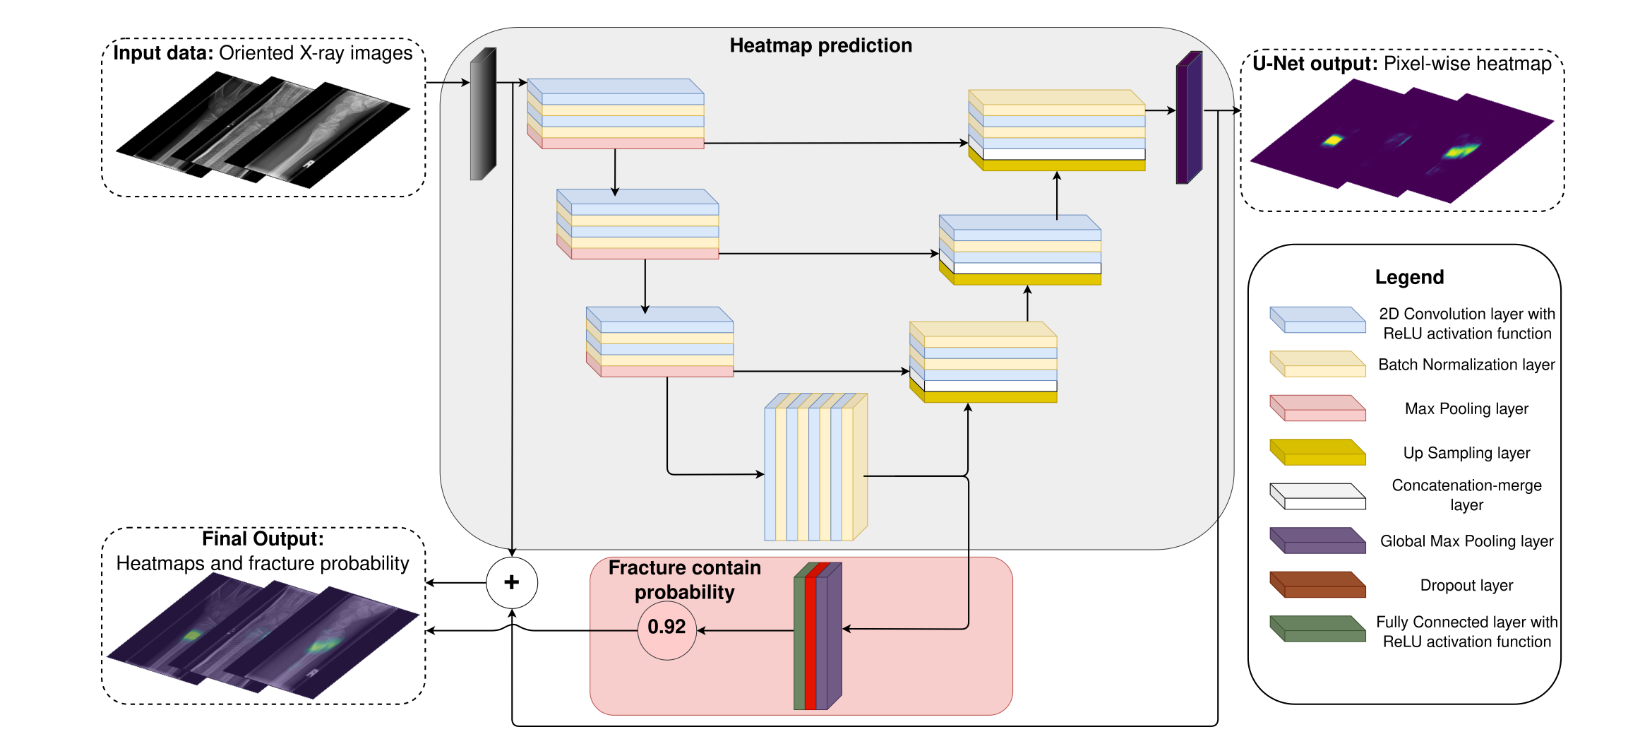
\includegraphics[width=1\textwidth]{images/unet.PNG}
	\caption{Minh họa về cấu trúc liên kết mô hình U-Net NN được sử dụng \cite{Lindsey1806905115}}
	\label{fig:unet}
\end{figure}

{\fontsize{13}{12} \selectfont

Để đạt được sự ổn định trong quá trình huấn luyện, đảm bảo hội tụ hàm mất mát trên tập dữ liệu, bên cạnh việc chính quy hóa L2 được đề xuất ban đầu $(\lambda = 10^{-5})$, nghiên cứu này đã áp dụng kích hoạt ReLU sau mỗi lớp tích chập (thay vì mọi lớp tích chập khác). Hơn nữa, sau mỗi lớp chập, thêm một lớp chuẩn hóa hàng loạt cũng giúp mô hình hội tụ trong quá trình huấn luyện. \cite{10.5555/3327144.3327174}.

Do giới hạn phần cứng, kích thước đầu vào của hình ảnh được đặt thành 512 × 512 (thay vì 1024 × 512). Kích thước lô được đặt thành 8. Hàm mất mát là tổng của hai hàm cross-entropy nhị phân (bản đồ nhiệt và xác suất đứt gãy) và bộ tối ưu hóa là Adam với tốc độ học $\alpha = 10^{-4}$ \cite{Buja2005LossFF}.


\begin{figure}[H]
\centering
	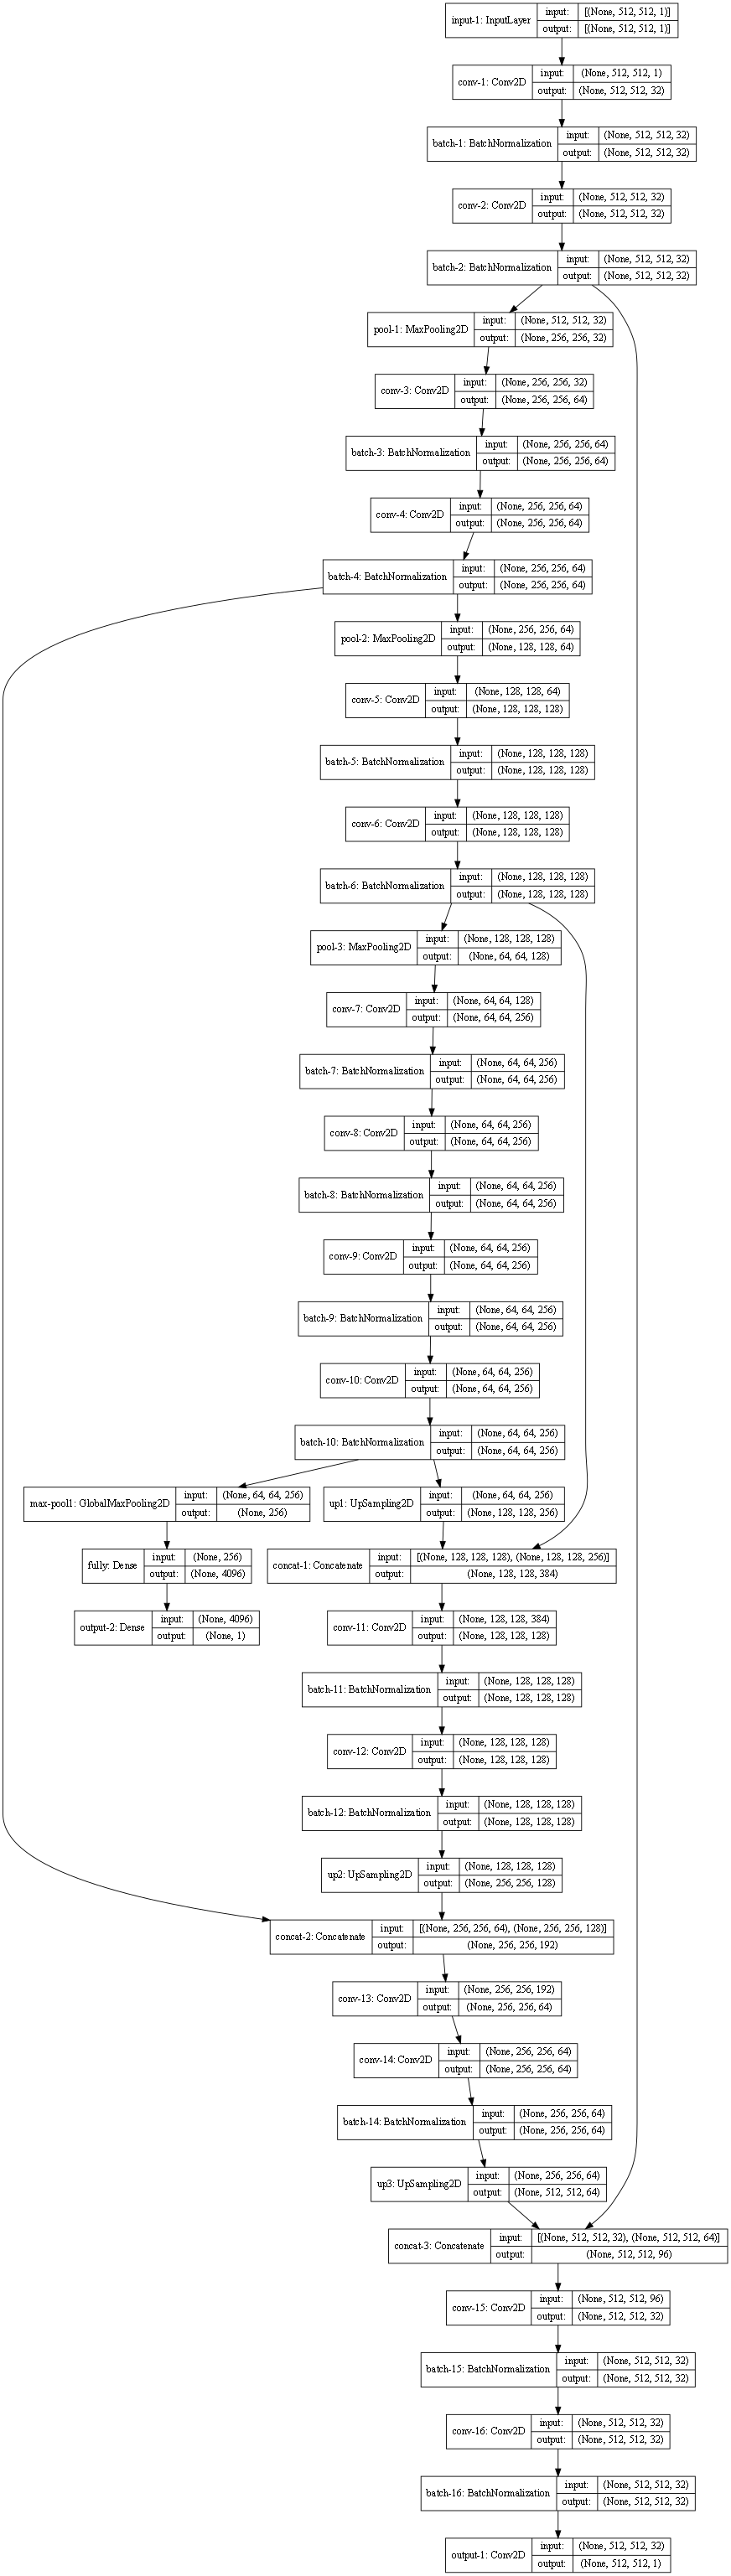
\includegraphics[width=0.4\textwidth]{images/model_unet.png}
	\caption{Mô tả chi tiết về các lớp của mô hình U-Net}
	\label{fig:model_unet}
\end{figure}

}

\subsection{Mô hình Yolov4}

{\fontsize{13}{12} \selectfont
Chi tiết về kiến trúc, quá trình xử lý của mô hình Yolov4 đã được mô tả ở Mục \ref{sec:yolov4}. Ở phần này sẽ trình bày thêm những chi tiết sau.

Bochkovskiy \etal. \cite{Bochkovskiy2020YOLOv4OS} đã tiến hành một cuộc so sánh rộng rãi - tiêu tốn thời gian và tài nguyên - của YOLOv4 với các mô hình hiện đại khác nhau để phát hiện đối tượng và thực hiện một cuộc tìm kiếm mở rộng cho cấu trúc liên kết tốt nhất của phương pháp đề xuất của họ. Do đó, nghiên cứu đã xem xét các phát hiện và sử dụng mô hình đạt được kết quả tốt nhất trong nghiên cứu của họ. Hơn nữa, nhiều bài báo đang so sánh YOLOv4 với các phương pháp phát hiện đối tượng có sẵn khác trong đó YOLOv4 đạt được hiệu suất tương tự hoặc tốt hơn \cite{s20174938,WU2020105742,9079965,Aly2021YOLOVA}. Điều này thúc đẩy việc sử dụng mô hình YOLOv4 trong nghiên cứu này. Quá trình phát hiện gãy xương trên ảnh X-quang với mô hình Yolov4 được trình bày trong Hình \ref{fig:yolov4_pro}.

\begin{itemize}
  \item Dữ liệu đầu vào - Bước này bao gồm việc nâng cấp và xử lý trước dữ liệu đầu vào (XAOM với tỷ lệ hình ảnh thành 512 × 512 và 608 × 608 điểm ảnh). Trong nghiên cứu này sử dụng các phương pháp tăng cường dữ liệu và kích thước hình ảnh tương tự như trong cấu hình của YOLOv4.

  \item Trích xuất đặc trưng - Trong nghiên cứu YOLOv4, các tác giả đã so sánh hiệu năng của một số mô hình CNN, trong đó mô hình CSPDarknet53 cho kết quả tốt nhất \cite{9150780}.
 
   \item Tổng hợp đặc trưng - Các tác giả đã thảo luận về một số kiến trúc mô hình để tổng hợp đặc trưng và quyết định sử dụng mô hình PANet \cite{8579011}. Trong nghiên cứu này cũng sử dụng PANet cho phần tổng hợp đặc trưng.
   
   \item Bộ phát hiện gãy xương - Tạo ra một véc tơ đại diện cho các đối tượng. Mỗi đối tượng được xác định với một mỏ neo (tọa độ của hộp giới hạn dự đoán: tâm, chiều cao, chiều rộng) và xác suất lớp.
\end{itemize}
}

\begin{figure}[ht!]
\centering
	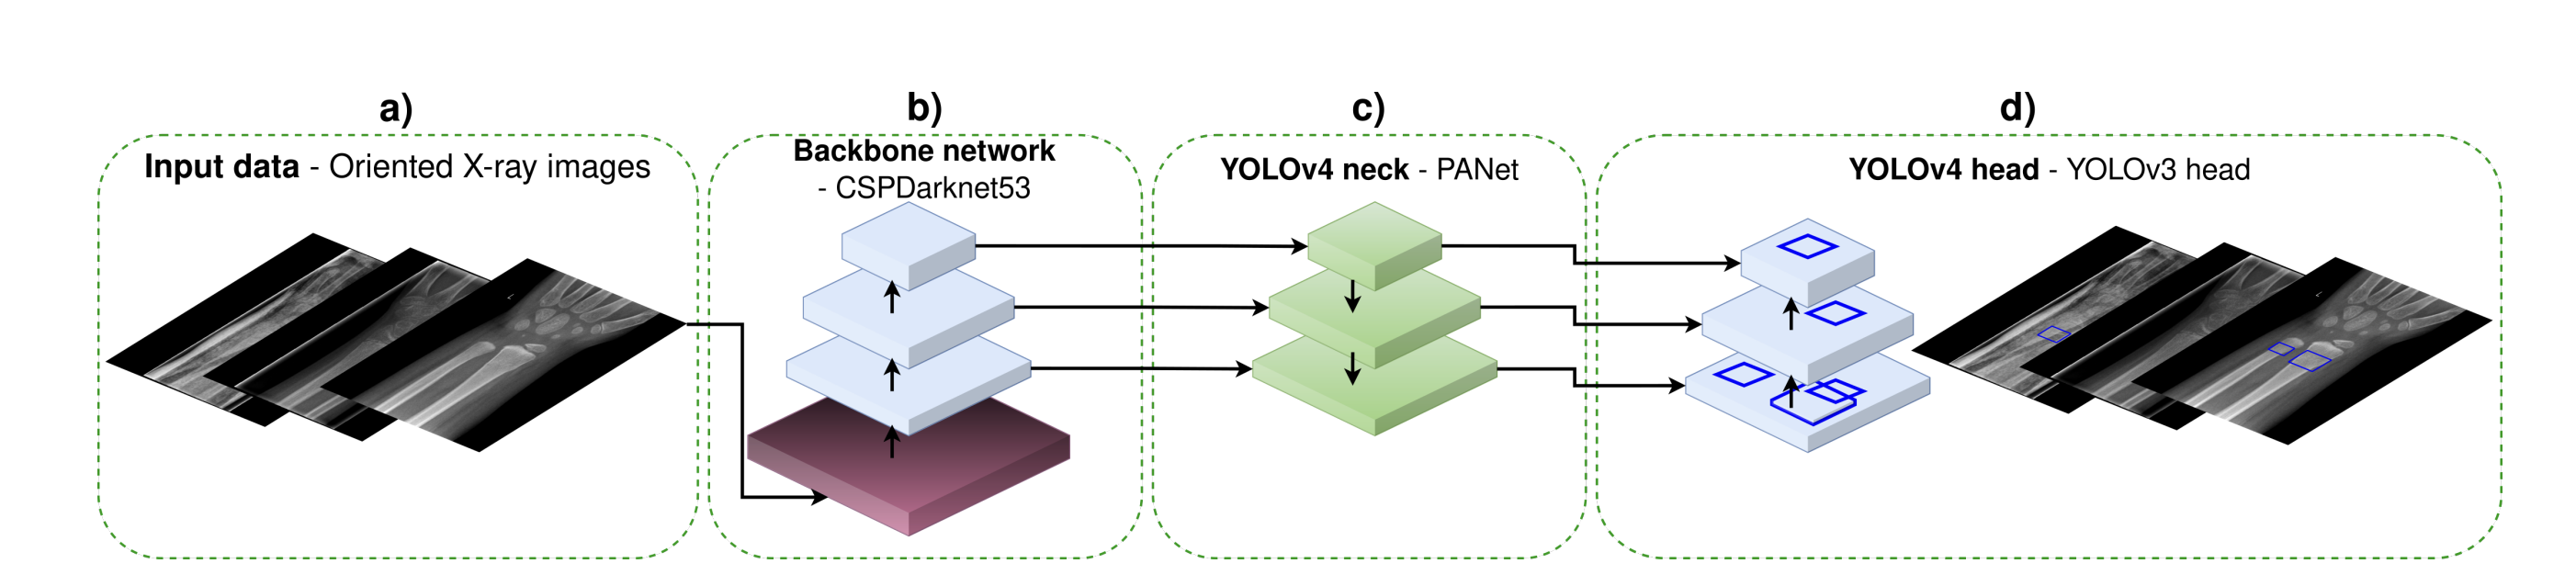
\includegraphics[width=1\textwidth]{images/yolov4_pro.png}
	\caption{Các bộ phận chính của YOLOv4. (a) Dữ liệu đầu vào được xử lý trước và tăng cường. (b) Mô hình CSPDarknet53 để trích xuất đặc trưng. (c) PANet để tổng hợp các đặc trưng. (d) Bộ phát hiện gãy xương}
	\label{fig:yolov4_pro}
\end{figure}

{\fontsize{13}{12} \selectfont
Ta có thể tăng độ chính xác của dự đoán lớp và diện tích hộp giới hạn ước tính bằng cách thiết lập các ước tính ban đầu về kích thước của mỏ neo. Ước tính kích thước của neo được hoàn thành bằng cách chạy thuật toán phân cụm k-means trên tập dữ liệu huấn luyện với số lượng cụm là 9 \cite{Likas2003}. Do đó, tổng cộng, đã huấn luyện và thử nghiệm bốn mô hình YOLOv4 để phát hiện gãy xương:

\begin{itemize}
  \item Mô hình YOLO 512 có kích thước hình ảnh đầu vào được đặt thành 512 × 512 và kích thước neo ban đầu: (12, 16), (19, 36), (40, 28), (36, 75), (76, 55), (72, 146), (142, 110), (192, 243), (459, 401).

  \item Mô hình neo YOLO 512 có kích thước hình ảnh đầu vào được đặt thành 512 × 512 và kích thước neo ước tính: (23, 22), (44, 27), (35, 40), (73, 31), (55, 41), (61, 62), (84, 47), (101, 67), (92, 115).
   
  \item Mô hình YOLO 608 có kích thước hình ảnh đầu vào được đặt thành 608 × 608 và kích thước neo ban đầu: (12, 16), (19, 36), (40, 28), (36, 75), (76, 55), (72, 146), (142, 110), (192, 243), (459, 401).
  
  \item Mô hình neo YOLO 608 có kích thước hình ảnh đầu vào được đặt thành 608 × 608 và kích thước neo ước tính: (40, 41), (70, 51), (109, 58), (82, 82), (157, 70), ( 122, 94), (114,155), (176,111), (206,176).
\end{itemize}

Tất cả các siêu tham số khác đều được sử dụng giống như trong nghiên cứu gốc ngoại trừ tốc độ học $\alpha$. Các siêu tham số như sau: trình tối ưu hóa là một đường đi xuống dốc ngẫu nhiên (SGD) với tốc độ học $\alpha = 0,0013$ được chọn giữa các giá trị được đề xuấtc: từ 0,01 đến 0,00261, và được nhân với hệ số 0,1 ở 80 lần huấn luyện, quán tính 0,949, phân rã 0,0005. Kích thước lô được đặt là 64 và phương pháp chính quy hóa là dropBlock với xác suất bỏ 0,1. PANet (mô-đun SPP) đã sử dụng các lớp tổng hợp tối đa với kích thước nhân $k \times k$, trong đó k = 1, 5, 9, 13. Hơn nữa, tất cả các mô hình được thử nghiệm đã được huấn luyện cho đến khi không có cải thiện đáng kể về độ chính xác. Thông thường, điều này xảy ra sau 100 đến 150 lần huấn luyện lặp đi lặp lại.
}


\section{Tập dữ liệu}
\label{sec:dataset}

{\fontsize{13}{12} \selectfont
Trong phạm vi nghiên cứu này sử dụng tập dữ liệu được chia sẻ từ nghiên cứu của Nagy \etal \cite{Nagy2022}. Tập dữ liệu bao gồm 20,327 hình ảnh X-quang cổ tay trẻ em được thu thập từ 6,091 bệnh nhân nhi. Tập dữ liệu được gán nhãn bởi nhiều sinh viên và bác sĩ thông qua công cụ trực tuyến Supervisely (Deep Systems LLC, Moscow, Nga) bằng cách khoanh vùng các vùng gãy xương. Ba bác sĩ nhi khoa được chứng nhận đã xác nhận tất cả các nhãn đã được gán chính xác. Các vị phát gán nhãn được điều chỉnh cho đến khi đạt được sự đồng thuận giữa các bác sĩ. Các bác sĩ X-quang nhi khoa được hội đồng chứng nhận có kinh nghiệm từ 6 đến 29 năm trong lĩnh vực X-quang cơ xương khớp đã xác nhận tất cả các vùng gãy xương trên hình ảnh X-quang là chính xác.

Trong Bảng \ref{tab:dataset} trình bày tổng quan về các đặc điểm của tập dữ liệu. Độ tuổi trung bình của bệnh nhân từ $10,09$, phân bố theo giới tính: 2.688 nữ, 3.402 nam, 1 chưa xác định.

}

\begin{table}[!ht]
	\centering
	\caption{Thuộc tính của tập dữ liệu}
	\begin{tabular}{|p{2cm}|p{4cm}|p{3.5cm}|p{2cm}|}
		\hline
		\multicolumn{1}{|l|}{
		\textbf{\#}} 
		& \multicolumn{1}{c|}{\textbf{Mô tả}} 
		& \multicolumn{1}{c|}{\textbf{Số lượng}} \\
		\hline
	
		 1
		& Mã phân loại AO 
		& 14.158 (69,65\%)\\
		\hline
		
		 2
		& Hình ảnh có bó bột 
		& 5.776 (28,42\%)\\
		\hline
		
		 3
		& Các hình ảnh chẩn đoán chưa chắc chắn 
		& 537 (2,64\%) \\
        \hline
        
		 4
		& Biểu hiện chấn thương ban đầu
		& 10.861 (53,43\%) \\
        \hline
        
		 5
		& Có cấy ghép kim loại
		& 708 (3,48\%) \\
        \hline
        
		 6
		& Có dấu hiệu loãng xương
		& 2.473 (12,17\%) \\
        \hline
        
		 7
		& Chế độ chụp AP
		& 10.086 (49,62\%) \\
        \hline
        
		 8
		& Chế độ chụp LAT
		& 10.148 (49,92\%) \\
        \hline
        
		 9
		& Chế độ chụp xiên
		& 93 (0,46\%) \\
        \hline
        
		 10
		& Hình chụp từ bên trái
		& 11.135 (54,78\%) \\
        \hline
        
		 11
		& Hình chụp từ bên phải
		& 9.192 (45,22\%) \\
        \hline
        
		 \textbf{Tổng cộng}
		& 
		& 20.327 (100,00\%) \\
		\hline
	\end{tabular}
	
	\label{tab:dataset}
\end{table}

{\fontsize{13}{12} \selectfont
Hơn nữa, trong Bảng \ref{tab:dataset} trình bày sự phân bố của các đặc điểm khác được trình bày trong hình ảnh, chẳng hạn như hình chiếu, mặt bên, sự hiện diện của vật đúc và sự hiện diện của kim loại. Chúng ta nên lưu ý rằng 9,573 nghiên cứu (94,3\%) có cả hình chiếu trước và sau. Không loại trừ bất kỳ loại hình ảnh nào, làm cho tập dữ liệu được sử dụng trở thành thách thức cho việc lập mô hình, nhưng vẫn thực tế trong thực hành lâm sàng thông thường.

Từ các hình ảnh có sẵn trong tập dữ liệu, nghiên cứu đã tạo bốn tập con rời rạc được lấy mẫu ngẫu nhiên:

\begin{itemize}
  \item Tập dữ liệu huấn luyện bao gồm 15,327 hình ảnh.

  \item Tập dữ liệu xác thực bao gồm 4,000 hình ảnh.
   
  \item Tập dữ liệu kiểm tra \#1, bao gồm 1,000 hình ảnh, được sử dụng để kiểm tra lần cuối các thuộc tính tổng quát hóa của mô hình.
  
\end{itemize}

Tóm lại, để đánh giá hiệu năng của phương pháp được đề xuất so với mô hình U-Net, nghiên cứu đã sử dụng tập hợp con dữ liệu huấn luyện, xác thực và thử nghiệm \#1 (tổng cộng 20,327 hình ảnh).

Để tiền xử lý dữ liệu, căn chỉnh hình ảnh sao cho các ngón tay luôn trỏ vào đường viền trên cùng của hình ảnh,  nghiên cứu đã tuân theo các nguyên tắc được đưa ra trong nghiên cứu của Lindsey \etal  \cite{Lindsey1806905115}. Phương pháp này này xuất hiện trong nhiều nghiên cứu liên quan đến phát hiện gãy xương cổ tay. Căn chỉnh và định hướng hình ảnh tia X được thực hiện bằng cách sử dụng XAOM \cite{HRZIC2021104300}. Vì hình ảnh có chất lượng cao, nên  nghiên cứu này không áp dụng phương pháp làm nhiễu nào.

Một vài hình ảnh ví dụ của tập dữ liệu được hiển thị trong các Hình \ref{fig:dataset_0}, \ref{fig:dataset_1}, \ref{fig:dataset_2}, và \ref{fig:dataset_3}.
}

\begin{figure}[H]
\centering
	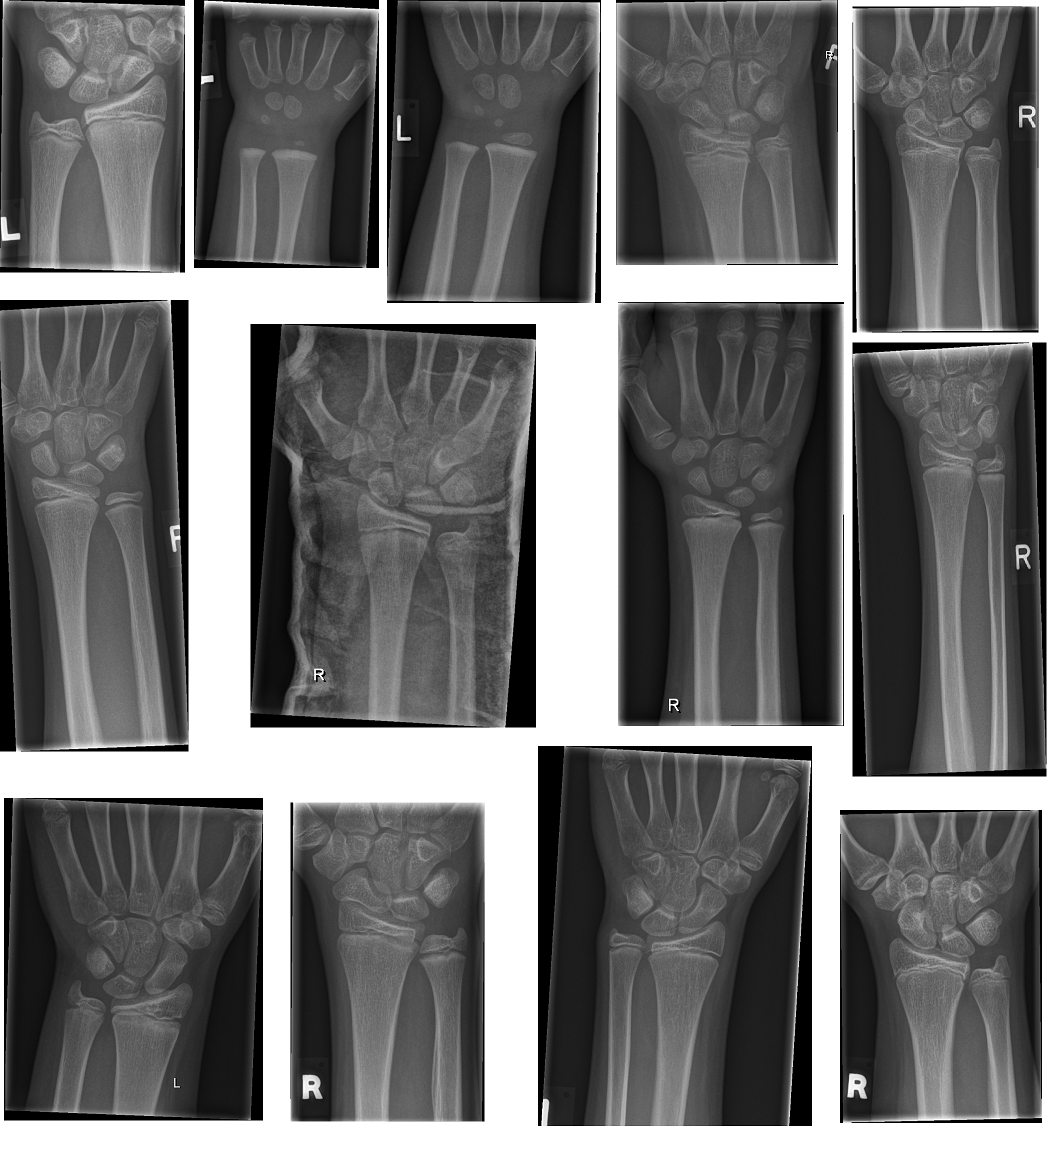
\includegraphics[width=1\textwidth]{images/dataset_0.png}
	\caption{Ví dụ về hình ảnh gãy xương trong tập dữ liệu - hình ảnh X-quang không chứa vết gãy xương.}
	\label{fig:dataset_0}
\end{figure}


\begin{figure}[H]
\centering
	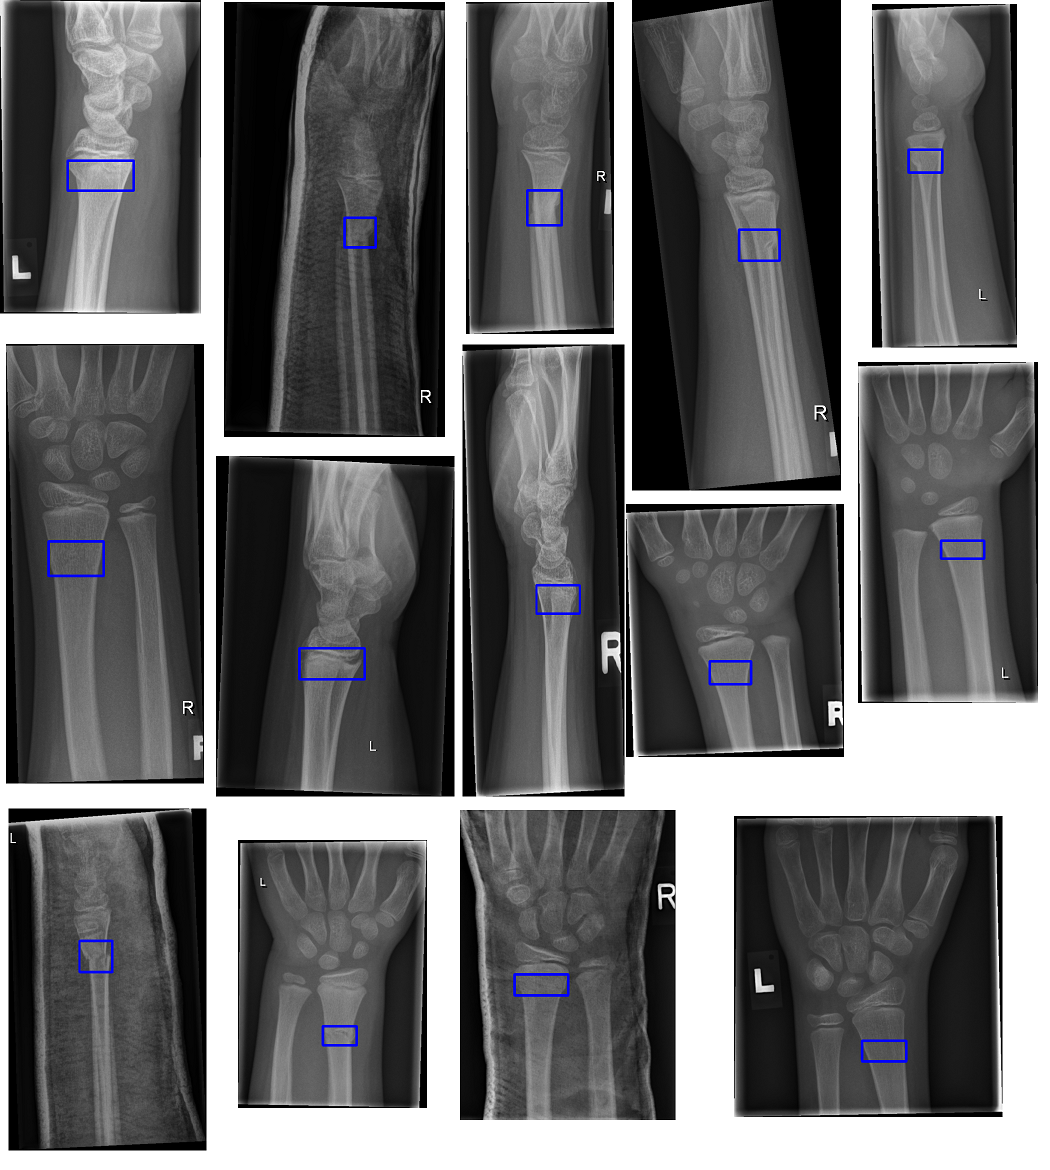
\includegraphics[width=1\textwidth]{images/dataset_1.png}
	\caption{Ví dụ về hình ảnh gãy xương trong tập dữ liệu - hình ảnh X-quang có chứa một vết gãy xương.}
	\label{fig:dataset_1}
\end{figure}

\begin{figure}[H]
\centering
	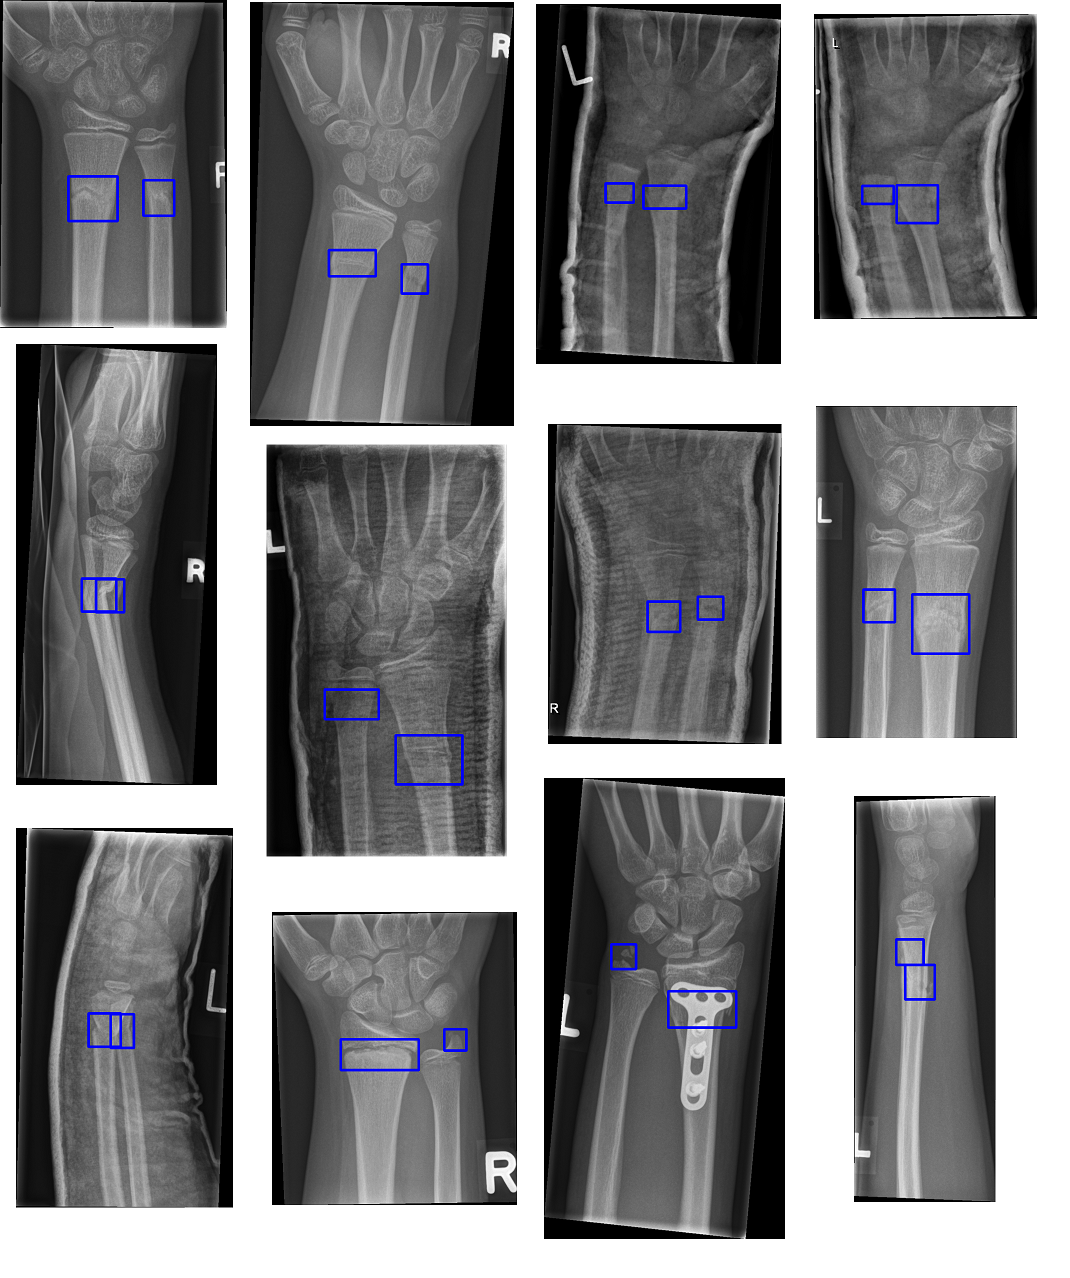
\includegraphics[width=1\textwidth]{images/dataset_2.png}
	\caption{Ví dụ về hình ảnh gãy xương trong tập dữ liệu - hình ảnh X-quang có chứa hai vết gãy xương.}
	\label{fig:dataset_2}
\end{figure}

\begin{figure}[H]
\centering
	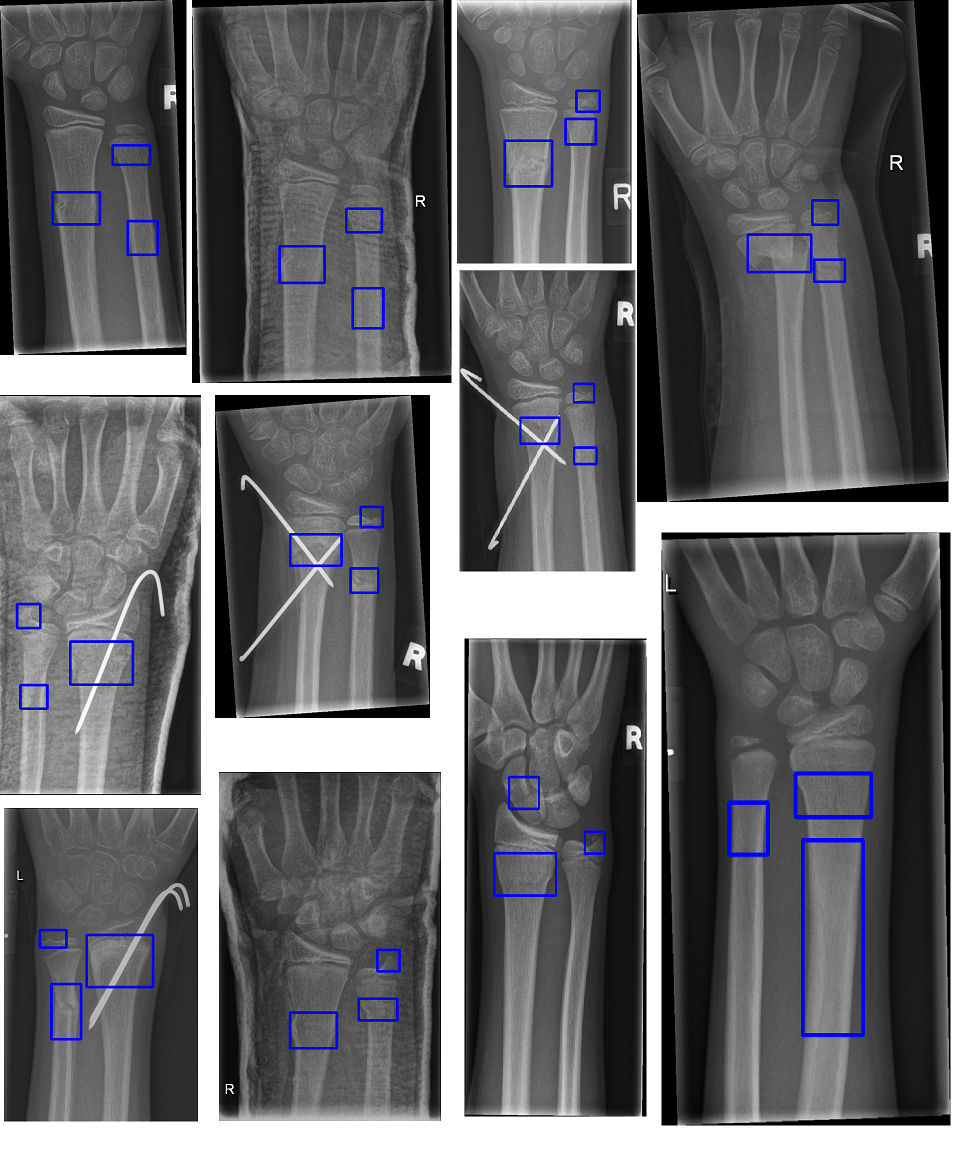
\includegraphics[width=1\textwidth]{images/dataset_3.png}
	\caption{Ví dụ về hình ảnh gãy xương trong tập dữ liệu - hình ảnh X-quang có chứa ba vết gãy xương}
	\label{fig:dataset_3}
\end{figure}

\section{Đánh giá hiệu năng}
\label{sec:eval}

\subsection{Các chỉ số để so sánh hiệu năng}

{\fontsize{13}{12} \selectfont
Độ chính xác của mô hình phát hiện gãy xương được xác định bởi chất lượng của việc khoanh vùng và phân loại đối tượng. Trong nghiên cứu này sử dụng các độ đo: độ chính xác, độ nhạy, F$_1$ và AUC-ROC. Ngoài ra, so sánh giữa giá trị dự đoán và nhãn để xác định vùng gãy xương, nghiên cứu cũng sử dụng độ đo IoU (Intersection over Union). 
}

\subsubsection*{Độ chính xác, độ nhạy và F$_1$}

{\fontsize{13}{12} \selectfont
Xét các định nghĩa sau:
\begin {itemize}
  \item True Positive (TP) thể hiện những giá trị dự đoán chính xác gãy xương.
  \item True Negative (TN) thể hiện các dự đoán chính xác không gãy xương.
  \item False Positive (FP) thể hiện các dự đoán nhầm về không gãy xương.
  \item False Negative (FN) thể hiện các dự đoán nhầm về gãy xương.
\end {itemize}

Công thức toán học của Precision và Recall được thể hiện lần lượt theo Công thức \ref{eq:precision} và Công thức \ref{eq:recall}. Precision và Recall có ý nghĩa khác nhau trong bài toán phát hiện đối tượng. Trong trường hợp muốn phát hiện nhiều đối tượng trong ảnh, chúng ta cần quan tâm đến giá trị Recall. Ngược lại, nếu muốn phát đối tượng chính xác hơn, ta nên cố gắng làm cho giá trị Precision càng lớn càng tốt. Do đó, hai giá trị này bị ràng buộc lẫn nhau. Điều đó có nghĩa là, khi giá tị Recall tăng lên, Precision sẽ giảm lại và ngược lại. Ngoài ra, giá trị F$_1$ là mức trung bình hài hòa giữa Precision và Recall (như trong Công thức \ref{eq:f1}).
}

\begin{equation}
    Precision = \frac{TP}{TP + FP}
    \label{eq:precision}
\end{equation}

\begin{equation}
    Recall = \frac{TP}{TP + FN}
    \label{eq:recall}
\end{equation}

\begin{equation}
    F_1 = 2 \times \frac{Precision \times Recall}{Precision + Recall} = \frac{2TP}{2TP + FP + FN}
    \label{eq:f1}
\end{equation}

\subsubsection*{IoU}

{\fontsize{13}{12} \selectfont
Số liệu IoU đo lường mức độ chính xác của một hộp giới hạn được dự đoán so với nhãn thật sự. 

Hình chữ nhật phía trên bên trái là nhãn và hình chữ nhật phía dưới bên phải là phần dự đoán. Vì kết quả phát hiện luôn khác với nhãn, IoU được xác định bằng cách chia giao điểm của phần dự đoán và nhãn cho phần kết hợp của chúng. Trong Yolo, ngưỡng IoU luôn được đặt là 0.5. Có nghĩa là, khi giá trị IoU của kết quả phát hiện lớn hơn 0.5, nó sẽ được coi là một TP. Khi giá trị IoU của kết quả phát hiện nhỏ hơn 0.5, nó sẽ được coi là một TN. Bằng cách điều chỉnh ngưỡng IoU, chúng ta có thể kiểm soát tỷ lệ TP và TN.
}

\begin{figure}[ht!]
\centering
	\includegraphics[width=1\textwidth]{images/IoU.PNG}
	\caption{Định nghĩa của IoU}
	\label{fig:IoU}
\end{figure}

\subsubsection*{Thử nghiệm McNemar}

Thử nghiệm McNemar \cite{McNemar1947} là một thử nghiệm đối với dữ liệu được ghép nối, như trong trường hợp bảng dự phòng $2 \times 2$ có đặc điểm lưỡng phân. Thử nghiệm McNemar xác định xem tần số hàng và cột biên có bằng nhau hay không, còn được gọi là tính đồng nhất biên. Thử nghiệm McNemar được thiết kế để tập trung chủ yếu vào sự khác biệt giữa hai mô hình, cụ thể là mỗi mô hình có thể sẽ cho một kết quả dự đoán khác nhau trên cùng dữ liệu đầu vào . Xét bảng dự phòng $2 \times 2$ với bốn ô trong đó mỗi ô và vị trí của nó được biểu thị bằng $n_{rc}$ trong đó $r$ là số hàng và $c$ là số cột. Giả sử ta có 2 mô hình A và B, xét các định nghĩa sau.

\begin {itemize}
  \item $n_{11}$ số lượng kết quả được phân loại sai bởi cả A và B.
  \item $n_{12}$ số lượng kết quả được phân loại sai bởi A nhưng không sai bởi B.
  \item $n_{21}$ số lượng kết quả được phân loại sai bởi B nhưng không sai bởi A.
  \item $n_{22}$ số lượng kết quả được phân loại đúng bởi cả A và B.
  \item Giả thuyết không ($H_0$): $n_{12}$ = $n_{21}$, có nghĩa là cả 2 mô hình A và B có tỉ lệ lỗi giống nhau.
\end {itemize}

Thử nghiệm McNemar về cơ bản là một dạng kiểm tra chi bình phương được ghép nối, vì vậy, tiếp theo chúng ta cần tính giá trị $X^2$ bằng Công thức \ref{eq:McNemar}.

\begin{equation}
    X^2 = \frac{(|n_{12} - n_{21}| - 1)^2}{n_{12} + n_{21}}
    \label{eq:McNemar}
\end{equation}

Khi kích thước mẫu của các ô $n_{12}$ hoặc $n_{21}$ nhỏ (thường được giả định là $n < 30$), một phép thử nhị thức có thể được sử dụng để tính toán thử nghiệm McNemar. Đây được gọi là bài kiểm tra điều kiện chính xác McNemar. Thử nghiệm một phía được định nghĩa theo Công thức \ref{eq:p_exact}

\begin{equation}
    p_{exact} = \sum_{i=n_{12}}^{n} \binom{n}{i} \frac{1}{2}^i (1 - \frac{1}{2})^{n-i}
    \label{eq:p_exact}
\end{equation}

\subsection{Các phương pháp đánh giá}

{\fontsize{13}{12} \selectfont
Để đánh giá hiệu suất mô hình một cách công bằng, nghiên cứu đã sử dụng ba cách đánh giá khác nhau trong tập thử nghiệm \#1.

\begin{itemize}
  \item Tiêu chuẩn đánh giá đầu tiên liên quan đến nhiệm vụ phân loại sự hiện diện gãy xương nhị phân (có / không). Do đó, gọi là đánh giá nhị phân. Đánh giá này được thiết kế theo nghiên cứu của Lindsey Lindsey \etal  \cite{Lindsey1806905115}. Bởi vì mô hình YOLOv4 xuất ra xác suất cho mỗi vết gãy được phát hiện,  nghiên cứu sẽ lấy xác suất gãy được phát hiện cao nhất trong một hình ảnh làm giá trị đầu ra. Đối với mô hình U-Net, chỉ cần lấy đầu ra từ phần thứ hai của nó. Để có được hiệu suất tốt nhất của các mô hình, nghiên cứu đã sử dụng ngưỡng xác suất chứa vết nứt $\gamma$ - nếu xác suất thấp hơn giá trị ngưỡng $\gamma$, nghiên cứu xác định không có vết gãy nào được trình bày trong hình ảnh.

  \item Tiêu chuẩn đánh giá thứ hai là đánh giá dựa trên hình ảnh. Trong thử nghiệm này sẽ đếm số lượng gãy xương được phát hiện trong hình ảnh. Cụ thể, một giá trị TP có nghĩa là số lượng vết gãy được phát hiện bởi mô hình giống với số lượng vết gãy thực tế trong hình ảnh. Nếu mô hình phát hiện nhiều hơn số lượng gãy xương thực tế, thì đó là một kết quả FP. Mặt khác, nếu nó phát hiện ra ít gãy xương hơn số gãy xương thực tế, thì đó là FN (nếu hình ảnh không có bất kỳ vết gãy nào và mô hình dự đoán số lượng gãy xương bằng không thì đó là TN). Đối với mô hình YOLOv4, đánh giá dựa trên hình ảnh rất đơn giản bởi vì sẽ thu được các hộp giới hạn, bao gồm các xác suất mà mỗi hộp giới hạn chứa một vết đứt gãy. Đối với mô hình U-Net, nghiên cứu phải phát triển một thuật toán để trích xuất hộp giới hạn (vùng). Thuật toán đầu tiên đặt bản đồ nhiệt thành ảnh trống đen (không có vết đứt gãy, xác suất bằng 0) nếu phần thứ hai của mô hình U-Net (xác suất chứa vết nứt) thấp hơn giá trị ngưỡng $\gamma$. Thứ hai, bản đồ nhiệt còn lại đại diện cho xác suất điểm ảnh của vết nứt được phân tích hai chiều bằng cách sử dụng một giá trị ngưỡng khác $\theta$. Cuối cùng, nghiên cứu ước tính các hộp giới hạn tối thiểu của các vết đứt gãy dựa trên các vùng còn lại của điểm ảnh màu trắng, sử dụng thuật toán lồi\cite{10.1145/235815.235821}. Mỗi hộp giới hạn đại diện cho một vết đứt gãy, điều này cho phép chúng ta đếm các vết đứt gãy bằng cách chỉ cần đếm các hộp giới hạn. Đánh giá dựa trên hình ảnh hoạt động đối với mô hình YOLOv4, nhưng nó không đánh giá đúng mô hình U-Net do các vấn đề được minh họa trong Hình. Cụ thể, sau khi áp dụng cả hai giá trị ngưỡng ($\gamma$ và $\theta$), một bản đồ nhiệt đôi khi sẽ được chia thành hai hộp giới hạn riêng biệt. Trường hợp ngược lại cũng xuất hiện khi dựa trên bản đồ nhiệt, chỉ phát hiện một hộp giới hạn, trong khi nhiều vết đứt gãy xuất hiện gần nhau. Một vấn đề khác là hộp giới hạn (sau khi áp dụng các giá trị ngưỡng) đôi khi sẽ khá nhỏ so với toàn bộ vùng bản đồ nhiệt, mặc dù toàn bộ bản đồ nhiệt hoàn toàn phù hợp với hộp giới hạn thực của một vết nứt. Do đó, đánh giá dựa trên hình ảnh nhằm mục đích cung cấp cho nghiên cứu ước tính sơ bộ về hiệu suất của các mô hình trong quá trình huấn luyện. Đối với hiệu suất của mô hình một cách chính xác nhất, nghiên cứu đề xuất đánh giá thứ ba.
   
  \item Thứ ba, và tiêu chuẩn đánh giá khắt khe nhất là đánh giá dựa trên gãy xương. Nếu hình ảnh có hai vết gãy, nghiên cứu sẽ có hai đánh giá cho hình ảnh cụ thể đó (một đánh giá cho mỗi vết gãy). Hình ảnh được xem là gãy xương nếu điểm IoU của hộp giới hạn dự đoán theo mô hình YOLOv4 và hộp giới hạn đứt gãy thực sự là cao hơn hoặc bằng 0.5, hoặc nếu bản đồ nhiệt được tạo ra bởi mô hình U-Net bị trùng lặp trên 50\% với vùng đứt gãy thực tế (bản đồ nhiệt không bị nhòe hơn 50\% đối với hộp giới hạn). Đối với đánh giá này, nghiên cứu cũng sử dụng ngưỡng $\theta$, bất kỳ vết gãy nào có xác suất nhỏ hơn giá trị ngưỡng đã đặt đều không được xem xét.

\end{itemize}

\begin{figure}[ht!]
\centering
	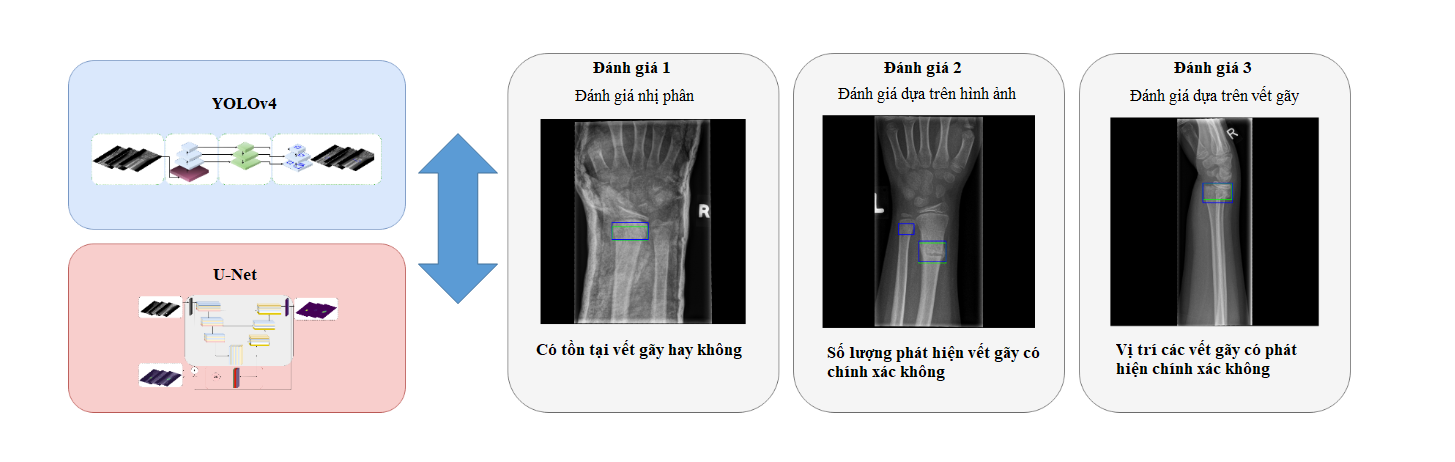
\includegraphics[width=1\textwidth]{images/eval.png}
	\caption{Minh họa về quy trình đánh giá mô hình.}
	\label{fig:model_eval}
\end{figure}

Hình \ref{fig:model_eval} mô tả một bản tóm tắt của quá trình đánh giá mô hình được thực hiện trong luận văn này.



}


\end{document}